% Grossly simplified system architecture -- high-level blocks only, laid out on
% the same geometry as system_architecture.tex (sim / perception / control
% stacked on the left, avoidance to the right, goal further right). No
% function/file/topic/node/command names. Single, axis-aligned arrows only;
% arrows carry a frequency where one is meaningful (MuJoCo step rate, command
% rate to the walking loop) -- no arrow carries a "quantity" label.
% Compile: pdflatex system_architecture_simplified.tex
\documentclass[tikz,border=10pt]{standalone}
\usetikzlibrary{positioning,arrows.meta,backgrounds,fit,calc}

\definecolor{nodeblue}{RGB}{31,119,180}
\definecolor{extgray}{RGB}{110,110,110}
\definecolor{goalgreen}{RGB}{34,120,44}

\begin{document}
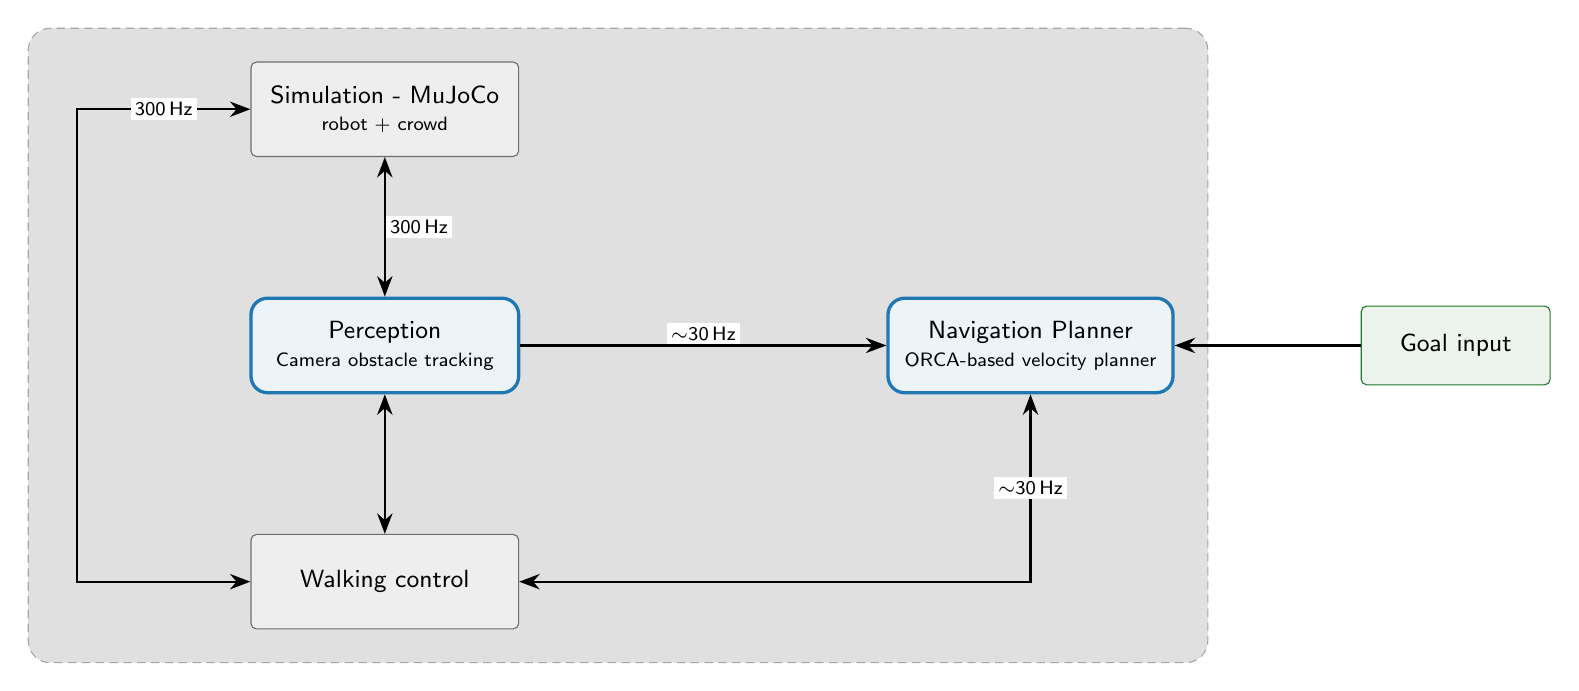
\begin{tikzpicture}[
  font=\sffamily\small,
  >={Stealth[length=2.6mm]},
  rosnode/.style={draw=nodeblue, very thick, rounded corners=6pt, align=center,
                  minimum height=12mm, minimum width=34mm, inner sep=6pt, fill=nodeblue!8},
  plain/.style={draw=extgray, rounded corners=2pt, align=center,
                minimum height=12mm, minimum width=34mm, inner sep=6pt, fill=extgray!12},
  goalbox/.style={draw=goalgreen, rounded corners=2pt, align=center,
                  minimum height=10mm, minimum width=24mm, inner sep=5pt, fill=goalgreen!8},
  arrow/.style={->, thick},
  biarrow/.style={<->, thick},
  lab/.style={font=\sffamily\scriptsize, align=center, fill=white, inner sep=1.5pt},
]

% ---------------- blocks (same coordinates as system_architecture.tex) ----------------
\node[plain]   (sim)    at (0,0)      {Simulation - MuJoCo\\[-1pt]\scriptsize robot + crowd};
\node[rosnode] (perc)   at (0,-3)     {Perception\\[-1pt]\scriptsize Camera obstacle tracking};
\node[plain]   (ctrl)   at (0,-6)     {Walking control};
\node[rosnode] (avoid)  at (8.2,-3)   {Navigation Planner\\[-1pt]\scriptsize ORCA-based velocity planner};
\node[goalbox] (goal)   at (13.6,-3)  {Goal input};

% ---------------- background shape: single in-process system ----------------
\coordinate (procpad) at ($(ctrl.west)+(-2.4,0)$);
\begin{scope}[on background layer]
  \node[rounded corners=8pt, draw=black!35, densely dashed, fill=black!12,
        inner sep=12pt, fit=(sim)(perc)(ctrl)(avoid)(procpad)] (proc) {};
\end{scope}

% ---------------- flow (all axis-aligned) ----------------
\draw[biarrow] (sim)  -- node[lab, right]{300\,Hz} (perc);
\draw[biarrow] (perc) -- (ctrl);
\draw[arrow] (perc) -- node[lab, above]{$\sim$30\,Hz} (avoid);
\draw[biarrow] (avoid.south) |- node[lab, pos=0.25]{$\sim$30\,Hz} (ctrl.east);
\draw[arrow] (goal) -- (avoid);
\draw[biarrow] (ctrl.west) -- ++(-2.2,0) |- node[lab, pos=0.75]{300\,Hz} (sim.west);

\end{tikzpicture}
\end{document}
